%______________________________________________________________________________________________________________________
% @briefLaTeX2e Resume for Kamil K Wojcicki
\documentclass[margin,line]{resume}
\usepackage[colorlinks = true,
linkcolor = blue,
urlcolor  = blue,
citecolor = blue,
anchorcolor = blue]{hyperref}

\usepackage[dvipsnames]{xcolor}
\usepackage{fontawesome}

\usepackage{etoolbox}
\BeforeBeginEnvironment{thebibliography}{%
  \let\origsection\section% save original definition of \section
  \let\section\subsection%  make \section behave like \subsection
}
\AfterEndEnvironment{thebibliography}{%
  \let\section\origsection% restore original definition of \section
}

\usepackage{fancyhdr}
\pagestyle{fancy}
\renewcommand{\headrulewidth}{0pt}
\newcommand{\COMMITHASH}{TRAVISCOMMIT}

\fancyhead{}
\fancyfoot{}
\lfoot{\hspace{-\sectionwidth} \href{{https://atlas-glance.cern.ch/atlas/membership/members/profile?id=9735}}{\faicon{link}~Giordon Stark's ATLAS Glance profile}}
\rfoot{\footnotesize Built \href{https://travis-ci.org/kratsg/cv/builds/\BUILDNUMBER}{\today} with \textcolor{red}{\faicon{heart}} for ATLAS Collaboration Board from \href{https://github.com/kratsg/cv/tree/\COMMITHASH}{\faicon{github} GitHub}}

\linespread{1.0}

%______________________________________________________________________________________________________________________
\begin{document}
\name{\Large \faicon{deaf} Giordon Stark {\small (pronouns: point/he/him)} \hspace{15.85em} 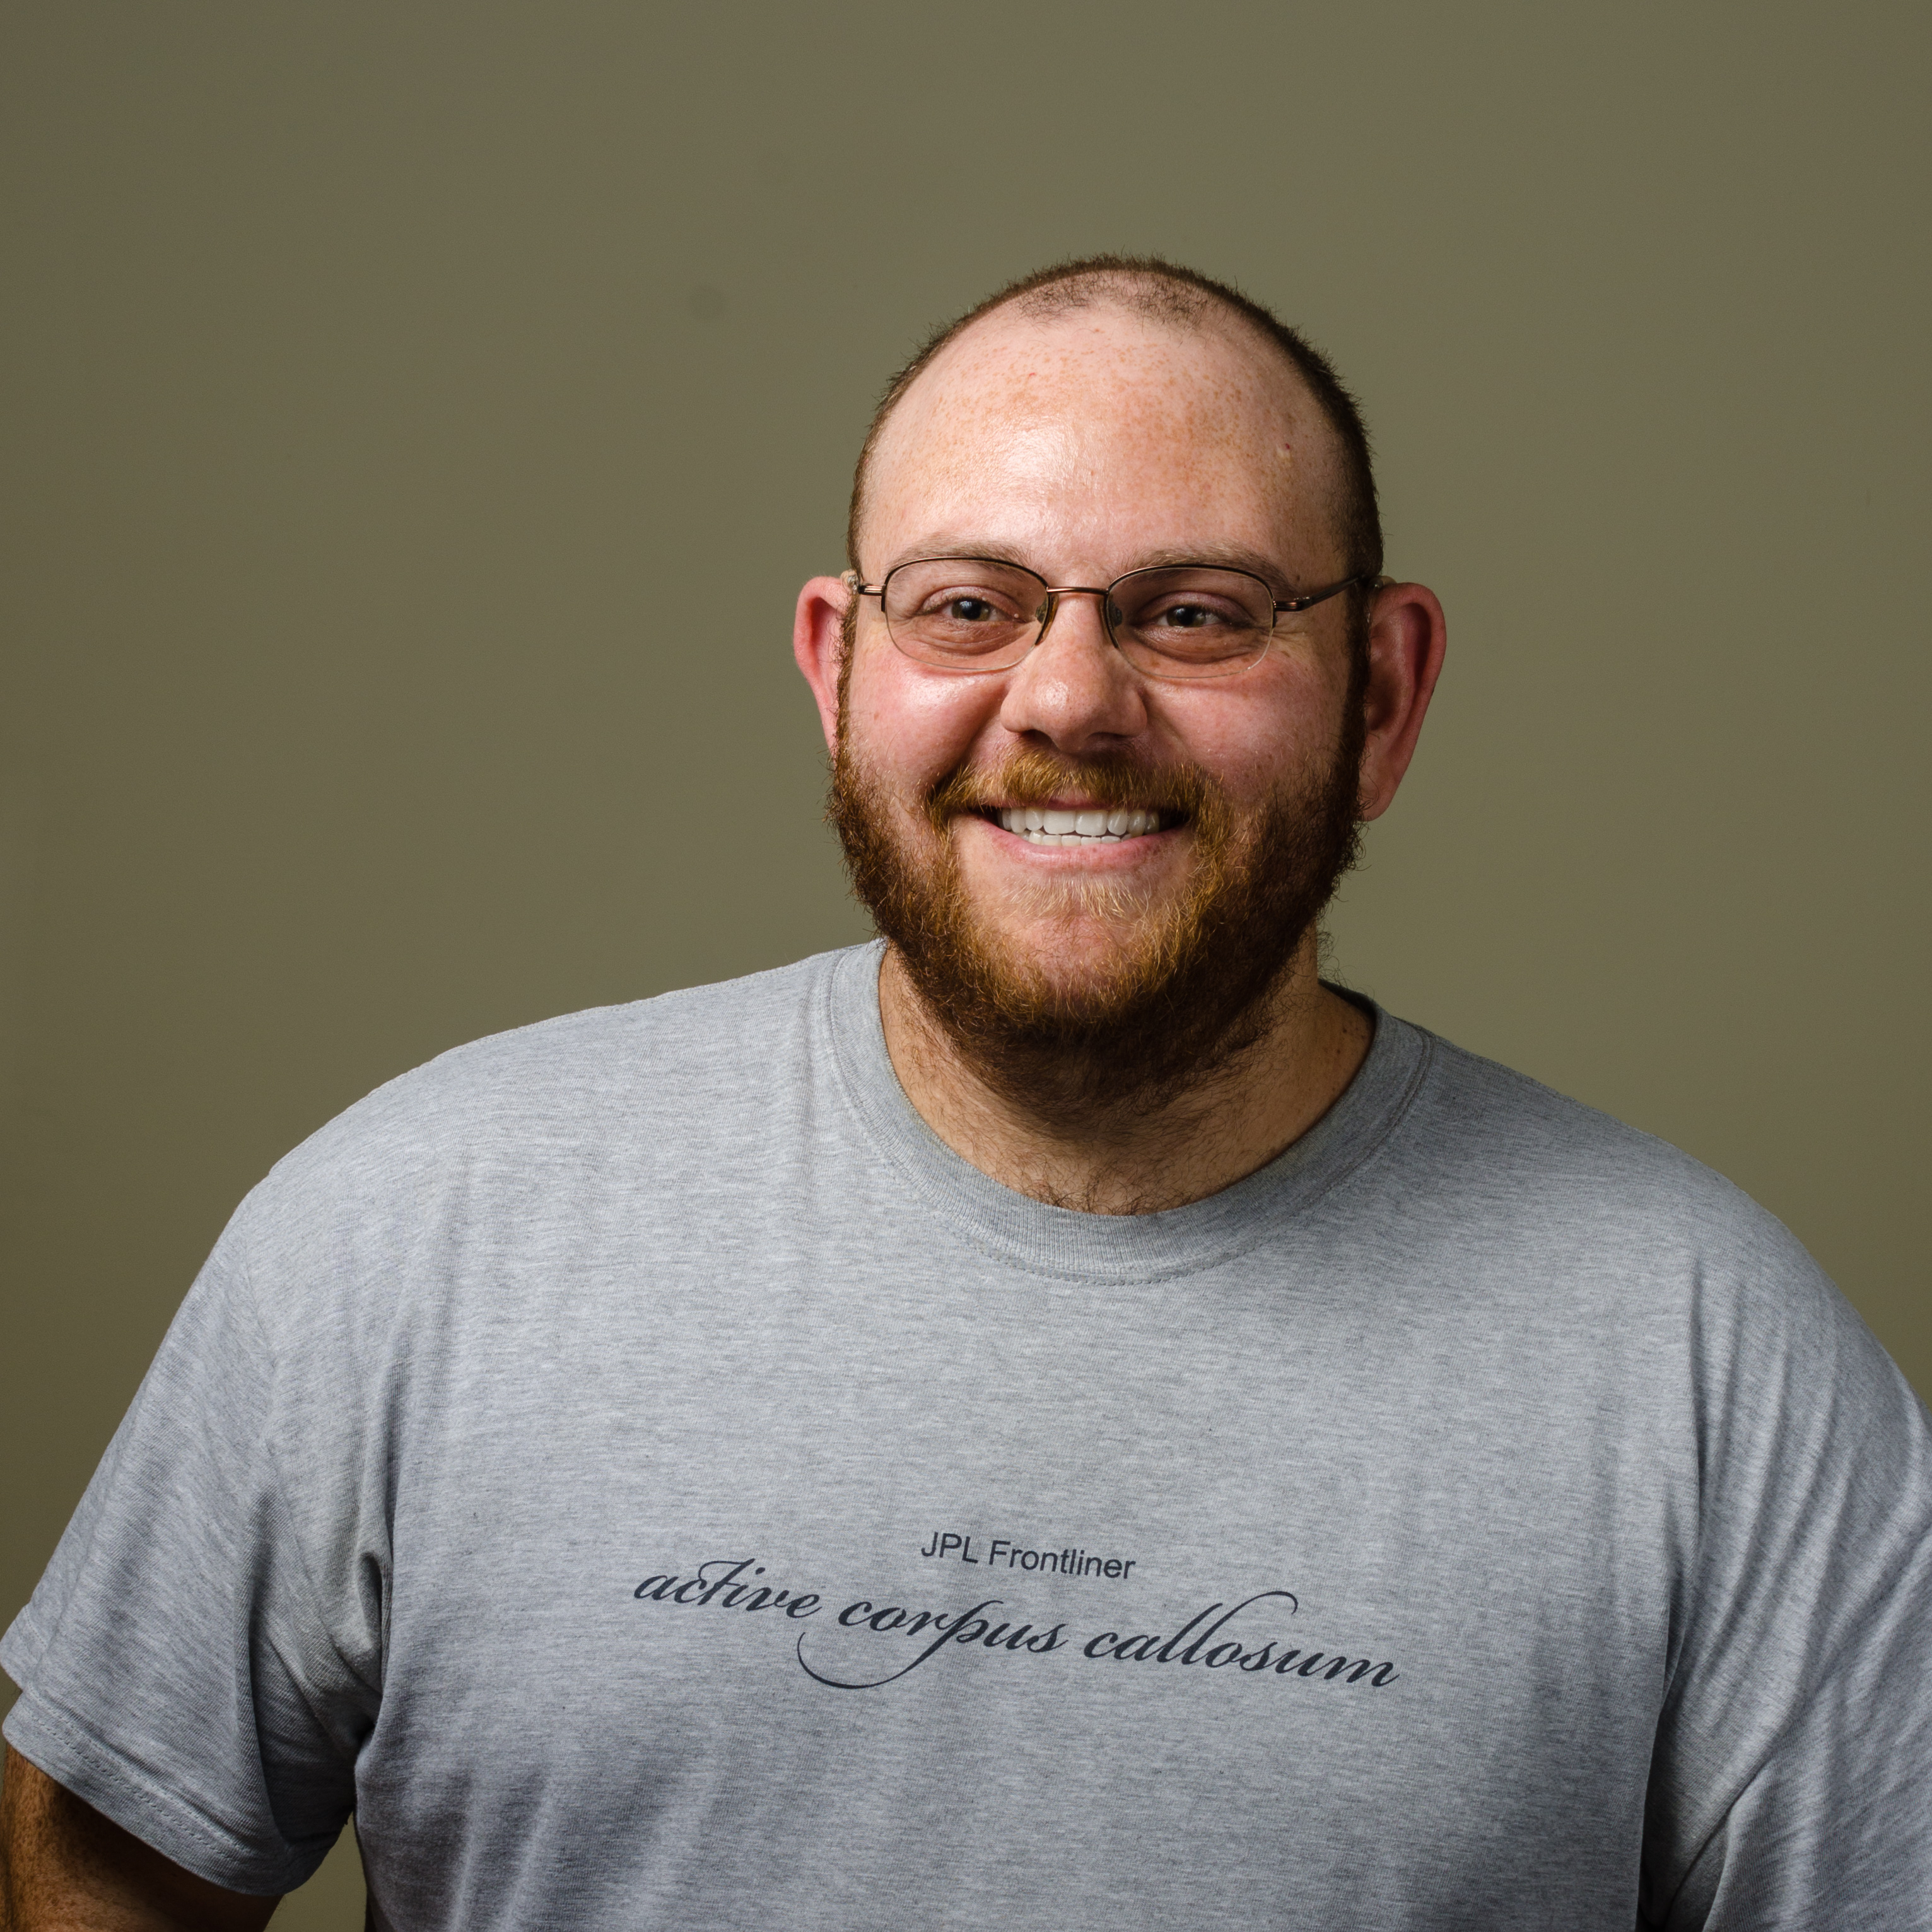
\includegraphics[width=2em]{figures/DSC_1436}}

\begin{resume}

%__________________________________________________________________________________________________________________
% Contact Information
\section{\mysidestyle Contact\\Information}

Giordon Stark                 \hfill \href{mailto:gstark@cern.ch}{\faicon{envelope}~gstark@cern.ch}
\vspace{0mm}\\\vspace{0mm}%
UCSC SCIPP, 1156 High Street  \hfill \href{https://github.com/kratsg}{\faicon{github}~kratsg} {\large\rmfamily\textbullet} \href{https://twitter.com/kratsg}{\faicon{twitter}~kratsg}
\vspace{0mm}\\\vspace{0mm}%
Natural Sciences 2, Room \#337       \hfill \href{https://orcid.org/0000-0001-6616-3433}{\faicon{key}~0000-0001-6616-3433}
\vspace{0mm}\\\vspace{0mm}%
Santa Cruz, CA \ \ \ 95064\hfill\href{https://giordonstark.com/?utm_source=cv}{https://giordonstark.com/}\\
\vspace{-6.5mm}%

%__________________________________________________________________________________________________________________
\section{\mysidestyle Academic History}

\textbf{SCIPP, UC Santa Cruz}, Santa Cruz, California \hfill \textbf{August 2018 -- present}\\
\textsl{Postdoctoral Scholar Employee}, Mike Hance
\begin{list2}
  \item Analysis Contact for Standard Model Collinear-W Measurement \hfill \textbf{November 2020 -- present}
  \item Organized the (virtual) USATLAS Computing Bootcamp \hfill \textsl{August 2020}
  \item SUSY Summaries subconvener \hfill \textbf{April 2019 -- present}
  \item ATLAS Open Likelihoods Developer/Advocate \hfill \textbf{September 2018 -- present}
  \item US ATLAS Diversity and Inclusion Committee \hfill \textbf{September 2018 -- present}
  \item ITk Pixel Instrumentation Upgrade efforts \hfill \textbf{August 2018 -- present}
  \item Contributing to various analyses in SUSY \hfill \textbf{March 2014 -- present}
  \item SUSY Common Dark matter ASG-RECAST Contact \hfill \textsl{March 2019 -- March 2020}
  \item SUSY Combinations Contact \hfill \textsl{October 2018 -- April 2020}
  \item SUSY Monte Carlo Produdction Contact \hfill \textsl{August 2018 -- July 2020}
  \item Instructor for many bootcamps and workshops to strengthen software expertise in HEP
  \item Recorded outreach videos for CERN and the \href{https://microcosm.web.cern.ch/en}{Microcosm exhibit} in American Sign Language. One video is on \href{https://www.youtube.com/watch?v=BaGjAruqFec}{YouTube}
\end{list2}
%
\textbf{University of Chicago}, Chicago, Illinois \hfill \textsl{September 2012 -- July 2018}\\
\textsl{Ph.D. Physics}, David Miller
\begin{list2}
  \item Lead analyzer for new physics search in SUSY Multi-\textsl{b}-jets \hfill \textsl{April 2017 -- April 2018}
  \item Editor of the gFEX Final Design Report \hfill \textsl{May 2016 -- April 2018}
  \item Advocated support for strong funding of U.S. HEP programs, based on\\ the P5 report, in Washington D.C. \href{https://www.usparticlephysics.org/strategy.html}{usparticlephysics.org} \hfill \textsl{2015}
  \item Bridge Program Tutor to enhance diversity in physics education \hfill \textsl{June 2014 -- April 2018}
  \item Worked to improve the ATLAS Trigger system in Run 3+ (gFEX)  \hfill \textsl{April 2014 -- April 2018}
  \item Qualification: gFEX Software/Firmware communications development \hfill \textsl{April 2014 -- April 2015}
  \item Graduate Student Teaching Assistant \hfill \textsl{June 2012 -- December 2017}
\end{list2}

%
\textbf{California Institute of Technology}, Pasadena, California \hfill \textsl{ Sep 2008 -- June 2012}\\
\textsl{B.S. Physics}, Kenneth Libbrecht and Harvey Newman

%__________________________________________________________________________________________________________________
\section{\mysidestyle Languages}

American Sign Language, English (bilingual), French Sign Language (elementary), British Sign Language (elementary), Italian Sign Language (elementary), Spanish (elementary), French (elementary)

%__________________________________________________________________________________________________________________
\section{\mysidestyle Dissertation}

\textbf{\textsl{Ph.D.}} \href{https://kratsg.github.io/thesis/?utm_source=cv}{\faicon{link}}~\textsl{The search for supersymmetry in hadronic final states using boosted object reconstruction}\\
ISBN: \href{https://books.google.com/books?vid=ISBN978-3-030-34548-8}{978-3-030-34548-8}\\[2.5mm]
\textbf{\textsl{B.S.}}\hspace{3mm} \href{https://www.dropbox.com/s/h0mpop96cn563bq/Thesis.pdf?dl=0}{\faicon{link}}~\textsl{Optical Coating Brownian Thermal Noise in Gravitational Wave Detectors}

%__________________________________________________________________________________________________________________
\section{\mysidestyle Honours and\\Awards}

Springer Thesis Award \hfill \textsl{August 2019}\\
Nathan Sugarman Award for Excellence in Graduate Student Research \hfill \textsl{May 2017}\\
US ATLAS Outstanding Graduate Student Award \hfill \textsl{June 2016}\\
Young Researchers' Symposium Award for Best Poster Presentation \hfill \textsl{November 2015}\\
Department of Energy, Office of Science Graduate Student Research \hfill \textsl{Oct. 2015 - Jan. 2016}\\
UChicago Excellence in Graduate Teaching nominee \hfill \textsl{April 2015}\\
US LHC Users Association Lightning Round winner \hfill \textsl{November 2014}\\
UChicago Excellence in Graduate Teaching nominee \hfill \textsl{April 2014}\\
UChicago Excellence in Graduate Teaching nominee \hfill \textsl{April 2013}\\
Caltech Excellent TA Award \hfill \textsl{2012}\\
Edward C. and Alice Stone Fellow \hfill \textsl{June 2010}

\end{resume}
\end{document}
